\documentclass[conf]{new-aiaa}
%\documentclass[journal]{new-aiaa} for journal papers
\usepackage[utf8]{inputenc}

\usepackage{graphicx}
\usepackage{tikz}
\usetikzlibrary{positioning}
\usepackage{amsmath}
\usepackage{float}
\usepackage[version=4]{mhchem}
\usepackage{siunitx}
\usepackage{subcaption}
\usepackage{longtable,tabularx}
\setlength\LTleft{0pt} 


\title{A Cooperative Framework for Autonomous  Landings of Quadrotors using Vision on a Moving UGV}

\author{Rishab Balasubramanian\footnote{Under graduate, Department of Instrumentation And Control Engineeering. Email: rishab.edu@gmail.com }}
\affil{NIT Trichy, Tiruchirappalli -- 620015, India. }
\author{P.B. Sujit\footnote{Associate Professor, Department of Electrical Engineering and Computer Science. Email: sujit@iiserb.ac.in}}
\affil{IISER Bhopal, Bhopal -- 462066, India. }



\begin{document}

\maketitle

\begin{abstract}
Unmanned ground vehicle (UGV) have been become popular for deploying and recharging quadrotors to achieve various persistent applications. In order to accurately land the UAV on the UGV efficient landing controller must be designed.   Further, a single UGV may need to service several quadrotors and hence the UGV and UAV need to coordinate with each other for landing and take-off. In this paper we present a State Dependent Riccati Equation (SDRE)-based landing guidance with vision in the loop and a cooperative scheduling scheme for sequential landing. Simulations results are presented to show the efficacy of the landing and scheduling for different trajectories.  

%In many unmanned aerial vehicles (UAV) scenarios, it is essential to generate flexible trajectory and target tracking algorithms to land on mobile platforms, which requires higher levels of autonomy. Autonomous landing is challenging due to the errors present in generated data arising from localization errors and external disturbances. In this paper we present a State Dependent Riccati Equation (SDRE)-based control strategy and show its robustness to disturbances while following a trajectory, and its ability to achieve fast and accurate landing on non-static targets. We then extend the problem to a vision-only based landing policy and show the controller's ability to perform well even with errors in measurements and limited information. Finally, we develop coordination strategies between the ground target and the UAVs to facilitate multiple UAV landing on the target as it follows a curving path. The proposed approach is evaluated using software-in-the-loop for different landing scenarios. Results show that our method achieves landing within 0.5m accuracy, with tunable trajectory parameters.

\end{abstract}

\section{Nomenclature}

{\renewcommand\arraystretch{1.0}
\noindent\begin{longtable*}{@{}l @{\quad=\quad} l@{}}
$W$ & World Frame\\
$B$ & Body Fixed Frame of the UAV\\
$x_{d}$ & position of the UAV along X axis in $W$\\
$y_{d}$ & position of the UAV along Y axis in $W$\\
$z_{d}$ & position of the UAV along Z axis in $W$\\
$v_{dx}$ & velocity of the UAV along X axis in $W$\\
$v_{dy}$ & velocity of the UAV along Y axis in $W$\\
$v_{dz}$ & velocity of the UAV along Z axis in $W$\\
$a_{dx}$ & acceleration of the UAV along X axis in $W$\\
$a_{dy}$ & acceleration of the UAV along Y axis in $W$\\
$a_{dz}$ & acceleration of the UAV along Z axis in $W$\\
$\phi_{d}$ & roll of UAV\\
$\theta_{d}$ & pitch of UAV\\
$\psi_{d}$ & yaw of UAV\\
$\omega_{d}$ & angular velocity of UAV about Z axis\\
$T$ & desired thrust\\
$\phi_{des}$ & desired roll of UAV\\
$\theta_{des}$ & desired pitch of UAV\\
$\omega_{des}$ & desired angular velocity for UAV about Z axis\\
$m$ & mass of UAV\\
$g$ & acceleration due to gravity\\
$x_{r}$ & position of the target along X axis in $W$\\
$y_{r}$ & position of the target along Y axis in $W$\\
$z_{r}$ & position of the target along Z axis in $W$\\
$v_{rx}$ & velocity of the target along X axis in $W$\\
$v_{ry}$ & velocity of the target along Y axis in $W$\\
$v_{rz}$ & velocity of the target along Z axis in $W$\\
$a_{rx}$ & acceleration of the target along X axis in $W$\\
$a_{ry}$ & acceleration of the target along Y axis in $W$\\
$a_{rz}$ & acceleration of the target along Z axis in $W$\\
$\psi_{r}$ & yaw of target\\
$\omega_{r}$ & angular velocity of target about Z axis\\
$R_{b}$ & rotation matrix corresponding to transformation from $B$ to $W$\\
$R_{w}$ & rotation matrix corresponding to transformation from $W$ to $B$\\

\end{longtable*}}

\section{Introduction}

% Use of UAV and UGV 
Small unmanned aerial vehicles like quadrotors are highly popular to conduct surveys. We are interested in using these vehicles for cargo delivery during these pandemic times like COVID-19, where the interaction between human needs to be minimized while ensuring  supply chain is maintained. This requires the UAV to take off from the cargo vehicle, deliver the package and return to the vehicle for landing. This sequence of function can be automated to delivery application. Another similar application could be habitat mapping or convoy protection. Further, if the UAV carrying vehicle is an UGV then the operation can be autonomous without any harm to humans while performing operations in disease prone regions or remote regions. 




% Bring TAS and siva papers and introduce the need for accurate landing and scheduling
Most of the works focus on either route planning problem for the UAV and the UGV to meet the requirements with minimal refueling locations \cite{maini2019cooperative,mathew2015planning,manyam2016path} or on robust  landing of the UAV on the UGV \cite{gautam2017autonomous,serra2016landing,ghommam2017autonomous}. In these two works, a single UAV is used for planning paths. The mission can be accomplish faster and cover large regions in the presence of multiple UAVs. However, with multiple UAVs, either the platforms needs to be multiple landing pads or in many cases they need share a single landing platform. In order to minimize logistics, the vehicles need to share a single lading platform and hence there is a need for the vehicles to coordinate with the UGV on the availability of the landing pad. The focus of this paper is to develop accurate landing controller for the quadrotors and also develop a cooperative mechanism between UAV and UGV to ensure sequential and safe landings.

% Literature review

\cite{herisse2012landing
saripalli2006landing
serra2016landing
ghommam2017autonomous
falanga2017vision
vlantis2015quadrotor
li2019fast
jfr2
Araar2017
campoy2
campoy1
7139490
drones2040034}


\cite{}


% contribution. 



% organization
The rest of the paper is organized as follows. The landing problem formulation is presented in Section \ref{sec:pf} and the SDRE-based landing controller is designed in Section  \ref{sec:sdre}. The cooperative strategy is described in Section \ref{sec:coop}. The evaluation of the proposed framework is carried out through simulations which is described in Section \ref{sec:results} and the conclusions are presented in Section \ref{sec:conclusions}.




\section{Problem Formulation}\label{sec:pf}
Consider a 3D UAV-target engagement situation as in Fig.\ref{fig:drone}. For accurate and safe landing, it is imperative to generate controller commands that are non-oscillatory and easy to compute. Simply put, the aim is to drive the UAV from its current co-ordinates $(x_{d},y_{d},z_{d})$ to the coordinates of the target $(x_{r}, y_{r}, z_{r})$ at each timestep, while simultaneously ensuring the relative velocities between the UAV and target approaches zero. That is:

\begin{equation}
\lim_{t\to \infty} x-x_{r} = y-y_{r} = z-z_{r} = v_{dx}-v_{rx} = v_{dy}-v_{ry} = v_{dz}-v_{rz} = 0 
\end{equation}

We represent the situation as an infinite horizon regulator problem where we desire for the errors in position and velocity between the target and UAV to diminish to zero. We take these errors in $B$ as our states for the regulatory system, which are used to issue the controller commands. The desired pitch ($\theta_{des}$), roll ($\phi_{des}$), thrust ($T$), and angular velocity ($\omega_{des}$) of the UAV are taken as inputs to the system, and are used to develop an optimal guidance strategy based on SDRE formulation assuming a decoupled form of control. The architecture of the control strategy is shown in Fig.\ref{fig:archi}, where develop only the SDRE control and vision algorithms in this paper. The PID algorithm used is the internal model from Arduplilot, which converts the thrust, roll, pitch, and z-angular velocity commands (4 parameters) to motor commands (4 commands). Thus we do not explicitly consider the UAV dynamics. 

\begin{figure}
	\centering
	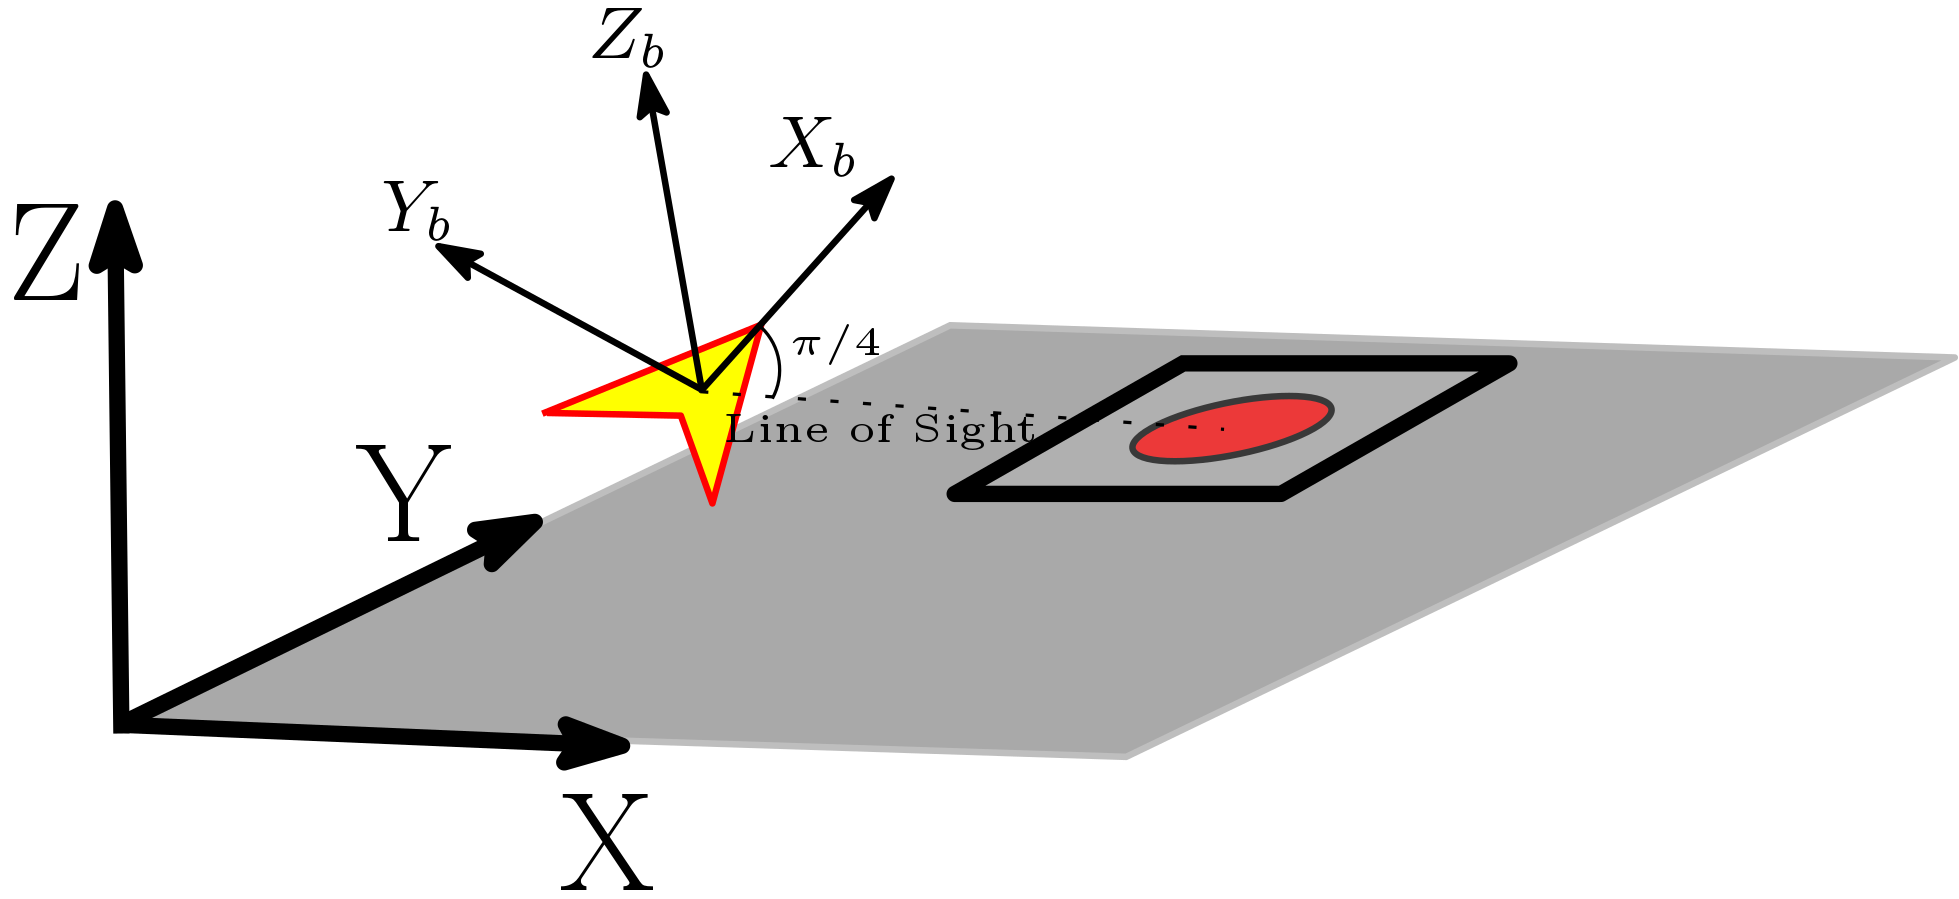
\includegraphics[scale=0.125]{drone.png}
	\caption{Representation of $W$ and $B$ frames, and the general landing problem}  \label{fig:drone}
\end{figure}

Let us define the errors in position and velocity between the target and UAV in $W$ as:
\begin{equation}
e_{q,ax}^{W} = r_{q,ax}^{W} - d_{q,ax}^{W}
\end{equation}
where q is the state used for error calculation (position or velocity), ax is the direction in $W$ (x, y, or z) and r and d represent the values for the rover and drone respectively. We then convert these parameters from $W$ to $B$ by:

\begin{equation}
\bar{e}_{q}^{B} = R_{w}\bar{e}_{q}^{W}
\end{equation}

where
\[
\bar{e}_{q}^{B} = \begin{bmatrix}
 e_{q,x}^{B}\\ e_{q,y}^{B}\\ e_{q,z}^{B}
\end{bmatrix}
\]
\[
\bar{e}_{q}^{W} = \begin{bmatrix}
 e_{q,x}^{W}\\ e_{q,y}^{W}\\ e_{q,z}^{W}
\end{bmatrix}
\]
\begin{equation}
R_{w} = 
\begin{bmatrix}
cos(\psi_{d})cos(\theta_{d}) & -sin(\psi_{d})cos(\phi_{d}) + sin(\phi_{d})sin(\theta_{d})cos(\psi_{d}) & sin(\psi_{d})sin(\phi_{d}) + cos(\phi_{d})cos(\psi_{d})sin(\theta_{d})\\
\\sin(\psi_{d})cos(\theta_{d}) & cos(\psi_{d})cos(\phi_{d}) + sin(\phi_{d})sin(\theta_{d})sin(\psi_{d}) & -sin(\phi_{d})cos(\psi_{d}) + sin(\psi_{d})sin(\theta_{d})cos(\phi_{d})\\
\\-sin(\theta_{d}) & cos(\theta_{d})\sin(\phi_{d}) & cos(\theta_{d})cos(\phi_{d})
\end{bmatrix}
\end{equation}
It is clear that
\begin{equation}
\dot{e}_{pos,ax} = e_{vel,ax}
\end{equation}
Therefore we shall here on refer to errors in positions along x, y, z in $B$ as $e_{x}, e_{y}, e_{z}$ and their respective error in velocity in $B$ as $\dot{e_{x}}, \dot{e_{y}}, \dot{e_{z}}$. We shall also define the error in yaw between the target and UAV as:
\begin{equation}
e_{\psi} = \psi_{r} - \psi_{d} 
\end{equation}

\begin{figure}[h]
  \centering
  \includegraphics[scale=0.35]{archi.png}
\caption{The figure shows the architecture of the control, feedback, and estimation model used.}  \label{fig:archi}
\end{figure}

Let us now turn our attention to the forces acting on the UAV. The only forces impacting the motion of the UAV are the weight, and thrust due to the rotors (not considering external forces due to wind or other disturbances). The thrust acts along the $z$ direction in $B$ and, gravity along $-z$ direction in $W$.
Thus the force due to gravity acting on the UAV in $W$ is:
\begin{equation}
Fg^{W} = \begin{bmatrix}
0 \\ 0 \\ -mg
\end{bmatrix}
\end{equation}
We get the force due to gravity in $B$ as:
\begin{equation}
Fg^{B} = R_{w}Fg^{W}\\
	   = \begin{bmatrix}
		mgsin\theta_{d} \\ -mgsin\phi_{d}cos\theta_{d} \\ -mgcos\phi_{d}cos\theta_{d}
		\end{bmatrix}
\end{equation}
Using small angle approximations, we get:
\begin{equation}
Fg^{B}= \begin{bmatrix}
		mg\theta_{d} \\ -mg\phi_{d} \\ -mg
		\end{bmatrix}
\end{equation}
Thus, the net force on the UAV in $B$ is:
\begin{equation}
F^{B}= \begin{bmatrix}
		mg\theta_{d} \\ -mg\phi_{d} \\ T-mg
		\end{bmatrix}
\end{equation}
where $T$ is the thrust due to the motors. We can find the acceleration of the UAV in $B$ by dividing $F^{B}$ by $m$. We shall assume here, we know the accelerations of the rover, and thus we can get the relative acceleration (error) between the target and quadrotor, which we define as our new virtual control inputs $u_{1}, u_{2}, u_{3}$:
\begin{equation}
e_{q, ax} = \begin{bmatrix}
a_{rx}-a_{dx} \\ a_{ry}-a_{dy} \\ a_{rz}-a_{dz}
\end{bmatrix} = \begin{bmatrix}
u_{1}\\
u_{2}\\
u_{3}
\end{bmatrix}
\end{equation}
where the virtual inputs are related to the real inputs as:
\begin{equation}
\theta_{des} = (a_{rx}-u_{1})/g
\end{equation}
\begin{equation}
\phi_{des} = (u_{2}-a_{ry})/g
\end{equation}
\begin{equation}
T = m(a_{ry}-u_{3})+mg
\end{equation}
Therefore we define our linearized state model in the form of:
\begin{equation}\label{eq:linear}
\dot{X} = A(X)X + B(X)U
\end{equation}
where:
\begin{equation}
X = \begin{bmatrix}
e_{x}\\
\dot{e_{x}}\\
e_{y}\\
\dot{e_{y}}\\
e_{z}\\
\dot{e_{z}}\\
e_{\psi}
\end{bmatrix}, 
A(X) = \begin{bmatrix}
0 & 1 & 0 & 0 & 0 & 0 & 0\\
0 & 0 & 0 & 0 & 0 & 0 & 0\\
0 & 0 & 0 & 1 & 0 & 0 & 0\\
0 & 0 & 0 & 0 & 0 & 0 & 0\\
0 & 0 & 0 & 0 & 0 & 1 & 0\\
0 & 0 & 0 & 0 & 0 & 0 & 0\\
0 & 0 & 0 & 0 & 0 & 0 & 0\\
\end{bmatrix},
B(X) = \begin{bmatrix}
0 & 0 & 0 & 0\\
1 & 0 & 0 & 0\\
0 & 0 & 0 & 0\\
0 & 1 & 0 & 0\\
0 & 0 & 0 & 0\\
0 & 0 & 1 & 0\\
0 & 0 & 0 & 1\\
\end{bmatrix},
U = \begin{bmatrix}
u_{1}\\
u_{2}\\
u_{3}\\
\omega_{des}\\
\end{bmatrix}
\end{equation}


\section{State Dependent Riccati Equation Control Law}\label{sec:sdre}
A general infinite time optimization problem can be defined as:
\begin{equation}
min\; J = \int_{0}^{\infty}X^{T}Q(X)X + U^{T}R(X)U
\end{equation}
where $X$ and $U$ are the states and inputs to our system respectively, related by \eqref{eq:linear}. The optimal control solution is given by:
\begin{equation}
    U^{*} = -R(X)^{-1} B(X)^T P X
\end{equation}
where $P$ is obtained by solving the Algebraic Riccati Equation (ARE)
\begin{equation}
    A(X)^T P + PA(X) - PB(X)R(X)^{-1} B(X)^T P +Q(X) = 0
\end{equation}

\subsection{Selection of Parameters in $Q(X)$ and $R(X)$}

The $R(X)$ and $Q(X)$ matrices are weight matrices which are chosen based on the application and information about the target available. Setting the diagonal elements in $R(X)$ with large values results in a rapid increase in cost $J$ as the input commands increase. This tends to ensure that the UAV does not tilt or rotate suddenly, and ensures smoother motion which is essential when tracking the target using vision based commands. However this restricts the aggressiveness of the UAV, and as a result it generates a limit to the speed of the target which can be tracked and landed upon by the quadrotor. The $Q(X)$ provides weights for the states in $X$. Again, there are a few considerations to be noted here. Firstly, we would like to descend as our errors in positions reduce, although not as rapidly, specifically in the case of vision-only landing. If the UAV descends too quickly, there is a high possibility it loses sight of the target, which results in landing failiure. Thus, the error in position along z should reduce slower than along x and y. Secondly, it is critical to penalize the error in velocity severley as the UAV approaches the target. This prevents overshoot, and allows for the UAV to match its speed with the target at the time of landing. Finally, we would also like to place suffiecient weightage on the error in heading for vision-based landing, as this allows us to track the rover from behind. As stated previously, to ensure we are constantly behind the rover, the error in velocity is heavily penalized. Once $R(X)$ is defined, we adjust $Q(X)$ so that we can acheive swift landing, without losing vision of the target (for the vision-based landing scheme). The $Q(X)$ and $R(X)$ matrices used, and considerations for choosing them are mentioned in subsequent sections.

\subsection{Stability Analysis}
We shall now consider the stability of the proposed controller. Let us define the function $f(X)$ as:
\begin{equation}
f(X)=AX
\end{equation}
Let us assume that the states are completely observable. Thus, from \cite{cimensdrestability}, we can say that the controller is locally stable about the origin if it satisfies
\begin{enumerate}
\item $f(X) \in C^{1}$
\item $f(0) = 0$
\item $B \neq \emptyset$
\item $\{A,B\}$ is controllable
\item $Q(X) \geq 0$ and $R(X) > 0$ 
\end{enumerate}

We will now prove the above conditions for the given controller
\begin{enumerate}
\item We can observe that:
\begin{equation}
f(X) = AX = \begin{bmatrix}
\dot{e_{x}}\\
0\\
\dot{e_{y}}\\
0\\
\dot{e_{z}}\\
0\\
0\\
\end{bmatrix} \in C^{1}
\end{equation}
\item When $X = 0$, 
\begin{equation}
f(X) = \begin{bmatrix}
0\\
0\\
0\\
0\\
0\\
0\\
0\\
\end{bmatrix}
\end{equation}
\item \begin{equation}
B = \begin{bmatrix}
0 & 0 & 0 & 0\\
1 & 0 & 0 & 0\\
0 & 0 & 0 & 0\\
0 & 1 & 0 & 0\\
0 & 0 & 0 & 0\\
0 & 0 & 1 & 0\\
0 & 0 & 0 & 1\\
\end{bmatrix} \neq \emptyset
\end{equation}
\item Let
\begin{equation}
Q_{c} = [B, AB, A^{2}B,...A^{6}B]
\end{equation}
We use MATLAB ctrb function to verify that the rank($Q_{c}$) = 7 = number of states.
\item This criteria is satisfied by choosing the diagonal elements of $Q$ and $R$ to be greater than 0. We shall observe that this is satisfied in the following sections, where the $Q$ and $R$ matrices are given for specific applications.
Thus the system is controllable
\end{enumerate}

\section{Baseline Control Model}
To test the full capabilities of the proposed controller, we assume that all the states in $X$ are completely observable. To do so we make the following assumptions:
\begin{enumerate}
\item The position, velocity, acceleration, heading and angular velocity of the target rover are known.
\item The position, velocity, acceleration, heading and angular velocity of the UAV is known.
\item The altitude at which the UAV is flying is known.
\item The rover moves along a horizontal plane
\item The height of the rover is known.
\end{enumerate}
Assumptions (1) and (2) are reasonable given that these states can be easily estimated using an Extended Kalman Filter over the data from GPS, IMU and odometry from each agent. Similarly a barometer can be used to estimate the altitude of the UAV for (3). While it is possible for to estimate the altitude of the rover using a barometer as well, we assume (4) for simplicity. The height of the rover from the ground is a property that is assumed to not vary, and can be measured before testing. We call this full state observable system as our Baseline control model, upon which we shall further develop.

To validate its working, we run simulation tests with the Baseline model, given the above assumptions. As we assume the system has complete observability, and prove the local stability of the controller, we can guarantee that, ideally, the UAV would land on the target. As a result we select the corresponding $Q(X)$ and $R(X)$ matrices to aggressively close the distance errors and then the velocity errors. The matrices used and results of the simulations are presented and discussed in Sec. \ref{sec:baseline_results}


\section{Position And Velocity Estimation Using Vision}\label{sec:vision}
To detect and track the target ground vehicle, a camera is mounted atop the UAV at an angle of $\pi/4$ with respect to the X axis in $B$, as in Fig \ref{fig:drone}. A grey colored landing space of dimension $1m\times1m$ is placed on top of the rover, on which a red colored target is attached. The input video from the camera is converted from RGB to HSV and YCrCb color spaces. This is because of the robustness of these color spaces to lighting conditions over RGB. In the HSV model, colors of each hue are arranged in a radial slice, around a central axis of neutral colors which ranges from black at the bottom to white at the top. Hue thus defines the dominant color of an area. The saturation dimension resembles various tints of bright color measuring the colorfulness, and the value dimension resembles luminance. The Hue, Saturation and Value are calculated as:
\begin{eqnarray}
H &=& \frac{\arccos(0.5(R-G)+(R-B))}{\sqrt{(R-G)^{2} + (R-B)(G-B)}},\\
S &=& 1-3\frac{\min(R,G,B)}{R+G+B}\\
V &=& \frac{R+G+B}{3}
\end{eqnarray}

\begin{figure}[t]
\begin{subfigure}{0.25\textwidth}
    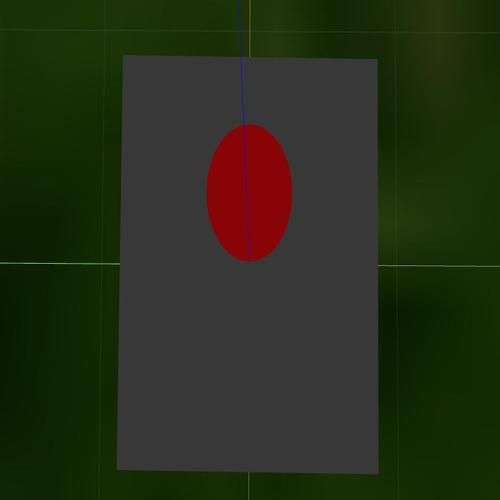
\includegraphics[width=\linewidth]{target2.jpg}
    \caption{} \label{fig:land_target}
  \end{subfigure}%
  \hspace*{\fill}   % maximize separation between the subfigures
  \begin{subfigure}{0.25\textwidth}
    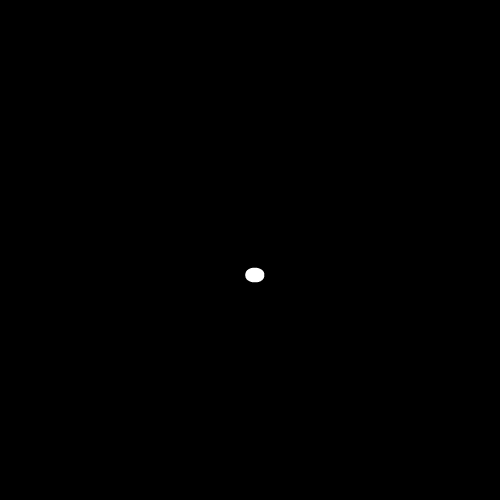
\includegraphics[width=\linewidth]{mask.png}
    \caption{} \label{fig:mask}
  \end{subfigure}%
  \hspace*{\fill}   
  \begin{subfigure}{0.25\textwidth}
    \includegraphics[width=\linewidth]{detect.png}
    \caption{} \label{fig:detect}
  \end{subfigure}%
  \hspace*{\fill} 
 \caption{a) The landing zone atop the rover with a red circular visual target b) Extracted mask of the red target c) The detected position of the target} \label{fig:vision_find}
\end{figure}

In the YCrCb color space the color is represented by luma Y, constructed as a weighted sum of RGB values, and two color difference values Cr and Cb that are formed by subtracting luma from RGB red and blue components.
\begin{eqnarray}
Y &=& K_{r}R + K_{g}G + K_{b}B,\\
Cr &=& R-Y,\\
Cb &=& B-Y.
\end{eqnarray}
In each computed color space, a mask is applied to remove only the regions which contain red colors. To remove noise, morphological transforms are used. The two resulting masks are then combined to obtain the final mask of the image. On this, blob detection algorithm is used to find the largest contour. The results are shown in Fig.\ref{fig:vision_find}. After blob detection, the center of the contour is calculated, and the coordinates received in pixel values are transformed to coordinates in the body fixed frame. There are several methods for doing this transformation, one of which is by using $K$ - the camera calibration matrix. However in this work, we use homography transformation and subsequent Single Value Decomposition (SVD) instead. To do this we make a few reasonable assumptions, similar to the previous section:
\begin{enumerate}
\item The target vehicle moves along a horizontal plane.
\item The altitude at which the quadrotor is flying is known to us.
\item The heading and angular velocity of the target vehicles is known. 
\item The target moves with a constant acceleration
\end{enumerate} 
Assumption (3) arises because of the use of color detection algorithms to estimate the position of the target. We can overcome this problem by using QR tags or Aruco markers to determine the orientation of the rover, but that is beyond the focus of this work. Assumption (4) is a major limitation to the vision-only based landing scheme. This can be overcome if the vision system is fused with data from the rover, to get a full state observable system, similar to the baseline model, or by using the cooperative strategy as proposed in Sec.\ref{sec:coop1}.
\subsection{Computing the Homography matrix}
We can define a transformation from image coordinates to global coordinates by using homographic transformations. Let us define the homographic matrix M as:
$$
M=
\begin{bmatrix}
m_{00} & m_{01} & m_{02}\\
m_{10} & m_{11} & m_{12}\\
m_{20} & m_{21} & m_{22}\\
\end{bmatrix},
$$
and $M^{'}$ as:
$$
M^{'}=
\begin{bmatrix}
m_{00}\\
m_{01}\\
m_{02}\\
m_{10}\\
m_{11}\\
m_{12}\\
m_{20}\\
m_{21}\\
m_{22}\\
\end{bmatrix}.
$$

Let the image co-ordinates be $(a_{1},b_{1})$ and the global co-ordinates be $(X_{1},Y_{1})$. Then we relate the two as:

$$
\begin{bmatrix}
a_{1}\\
b_{1}\\
1\\
\end{bmatrix}
\approx
\begin{bmatrix}
wa_{1}\\
wb_{1}\\
w1\\
\end{bmatrix}
=
M
\begin{bmatrix}
X_{1}\\
Y_{1}\\
1\\
\end{bmatrix}.
$$

To solve for the homography matrix, we use five directional vectors, in $B$ that correspond to (0,0), (w,0), (0,h), (w,h), (w/2, h/2) in the image frame, where w and h are the width and height in pixels of the image. These vectors are multiplied with the rotational matrix, $R_{w}$ to obtain the directional vectors in the world frame. Once the directional vectors are found in the world frame, their intersection with the $z=z_{r}$ plane is computed. Consider the intersection points as $(X_{i}, Y_{i}, z_{r})$ and the corresponding image coordinate as $(a_{i},b_{i})$. The matrix C is then computed using each point $i$ as follows: 
\begin{equation}
C=
\begin{bmatrix}
X_{i} & Y_{i} & 1 & 0 & 0 & 0 & -a_{i}X_{i} & -a_{i}Y_{i} & -a_{i}\\
0 & 0 & 0 & X_{i} & Y_{i} & 1 & -b_{i}X_{i} & -b_{i}Y_{i} & -b_{i}\\
\vdots & \vdots & \vdots & \vdots & \vdots & \vdots & \vdots & \vdots & \vdots\\
\end{bmatrix}.
\end{equation}

Once generated the entries of the homography matrix are then computed by solving the homogeneous equation:
\begin{equation}
CH^{'}=0.
\end{equation}
This can be done by using Singe Variable Decomposition (SVD). Once the homography matrix is determined, the image coordinates can be transformed to determine the position of the target relative to the UAV as:

\begin{eqnarray}
    e_{x}^{W} &=& \frac{(m_{00}a + m_{01}b + m_{02})}{(m_{20} + m_{21} + m_{22})},\\
    e_{y}^{W} &=& \frac{(m_{10}a + m_{11}b + m_{12})}{(m_{20} + m_{21} + m_{22})},
\end{eqnarray}
where $(a,b)$ is the pixel coordinates of the center of the red part of the target.

\subsection{Kalman Filter}
A Kalman Filter is now applied over the coordinates obtained from the vision system. Lets say that our prediction of the rover's next states $\hat{X}_{k+1}$, based on current data is given as:
\begin{equation}
    \underbrace{
    \begin{bmatrix}
    x_{k+1}\\
    v_{x_{k+1}}\\
    y_{k+1}\\
    v_{y_{k+1}}\\
    \end{bmatrix}
    }_{\hat{X}_{k+1}}
     = 
    \underbrace{\begin{bmatrix}
    1 & dt & 0 & 0\\
    0 & 1 & 0 & 0\\
    0 & 0 & 1 & dt\\
    0 & 1 & 0 & 1\\
    \end{bmatrix}}_\text{F}
    \underbrace{\begin{bmatrix}
    x_{k}\\
    v_{x_{k}}\\
    y_{k}\\
    v_{y_{k}}\\
    \end{bmatrix}}_{X_{k}}
\end{equation}
where $k+1$ denotes the next time step and $x, v_{x}, y, v_{y}$ denote the expected position and velocity of the target relative to the UAV along the X and Y axis in $W$ respectively. $F$ is the co-efficient matrix, $X_{k}$ is the previous states and $\hat{X}_{k+1}$ is the prediction matrix. Then the new expected covariance matrix $\hat{P}_{k+1}$ is:
\begin{equation}
    \hat{P}_{k+1} = FP_{k}F^T + Q_{k}
\end{equation}
where $P_{k}$ is the co-variance of the filter output and $Q_{k}$ is the noise matrix for the filter. Let the mean of the measured data be $Z_{k}$ and the noise covariance be $R_{k}$, which we can define as:
\begin{eqnarray}
    Z_{k+1} = H_{k}X_{k}\\
    R_{k+1} = H_{k}X_{k}H_{k}^{T}
\end{eqnarray}
where $H_{k}$ is the sensor matrix. The Kalman gain is then computed as:
\begin{equation}
    K = \hat{P}_{k+1}(\hat{P}_{k+1}+R_{k+1})^{-1}
\end{equation}
The new states $X_{k+1}$ and co-variance $P_{k+1}$ are thus calculated as:
\begin{eqnarray}
    X_{k+1} = \hat{X}_{k+1} + K(Z_{k+1} - \hat{X}_{k+1})\\
    P_{k+1} = \hat{P}_{k+1}(1-K)
\end{eqnarray}
Fig. \ref{fig:kalman} shows the results of the Kalman based prediction system. We can observe that although the prediction in target position is quite stable, the prediction in its velocity is oscillatory. This is caused by the oscillations of the UAV during its motion.

\begin{figure}[htb]
\begin{minipage}{0.5\textwidth}
\begin{tikzpicture}
  \node (img)  {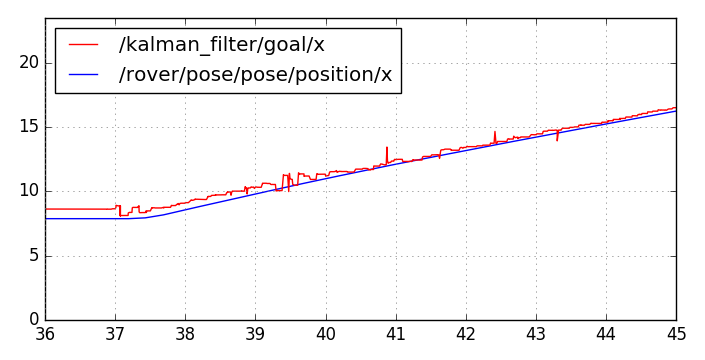
\includegraphics[scale=0.4]{position.png}};
  \node[below=of img, node distance=0cm, yshift=1.25cm,font=\color{black}] {time};
  \node[left=of img, node distance=0cm, rotate=90, anchor=center,yshift=-1.0cm,font=\color{black}] {Position};
 \end{tikzpicture}
\end{minipage}%
\begin{minipage}{0.5\textwidth}
\begin{tikzpicture}
  \node (img)  {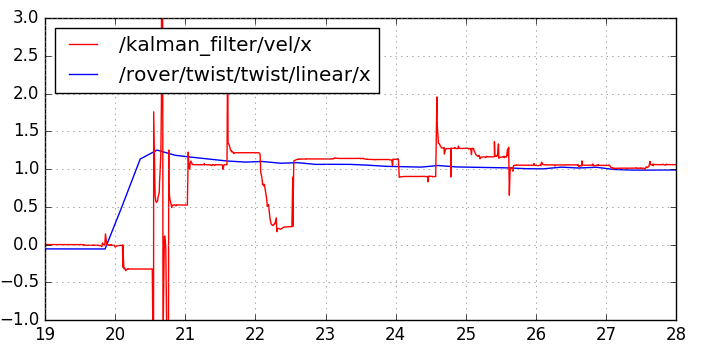
\includegraphics[scale=0.4]{velocity.png}};
  \node[below=of img, node distance=0cm, yshift=1.25cm,font=\color{black}] {time};
  \node[left=of img, node distance=0cm, rotate=90, anchor=center,yshift=-1.0cm,font=\color{black}] {Velocity};
\end{tikzpicture}
\end{minipage}%
\caption{The estimated position and velocity as the rover moves along the X axis with a speed of 1m/s} \label{fig:kalman}
\end{figure}


\section{Cooperative Strategy}\label{sec:coop}
We saw in Sec.\ref{sec:vision}, the biggest limitation of vision-based landing: landing on an accelerated target. We refer the reader to Fig.\ref{fig:oscillate_vision} where the quadrotor faces difficulties landing on a veering target. We also point the reader to Fig.\ref{fig:fail}, which shows the dangers and difficulties of landing on a swerving target, even with full observability. Such trajectories are extremely difficult to land upon, not only because of prediction and localization errors, but also because of their sharp changes in accelerations and velocities, which are difficult to match at the time of landing. Even with heading estimations of the target with QR tags or Aruco markers, the visibility of such visual aids in diverse lighting conditions is questionable, which seriously hinders the ability of the vision-only model to land on targets which are moving along suddenly curving trajectories. Here we put forth a solution to this problem using a coordination strategy between the aerial and ground vehicles. We also extend the proposed strategies to a multi-UAV setting. Here, it is imperative that the UAVs land on the target sequentially, without collisions. These call for a master-slave communication setup, where the target tells a particular UAV when it can land. In this section we present these cooperative strategies, and a method to implement them.
\subsection{Cooperative Strategy For Swerving Targets}\label{sec:coop1}
We begin by assuming that there exists some method of communication through which a message can be transmitted from the target to the UAV. One such example is vision-based communication, where the color of the landing pad can be changed from red to another color (e.g blue), depending on whether the target would like for the UAV to land on it or not. The rover acts as the master, and the UAVs as slaves during this phase. Let us call this transmitted data as $flag$. The rover, while following a desired path, changes the value of $flag$, based on whether it is safe for the UAV to land or not. In this paper, we consider it unsafe to land when the rover is turning, and safe to land when the rover moves along an approximate straight line. To test the suggested method, in some cases, we also term landing on the target during a particular part of its motion as "unsafe". However the notion of "safetiness" can vary based on the applicaiton. This $flag$ is then used by the UAV(s) to transition between hovering-tracking and landing modes. During the hovering-tracking mode, the UAV stays behind the target and tracks it, while maintaining it's current altitude. In the landing mode, the UAV decends onto the target. The results for this landing strategy is presented in Sec.\ref{sec:coop1_results}.

\subsection{Cooperative Strategy For Multi-UAV Landing}\label{sec:coop2}
In this setup, we have multiple UAVs wanting to land on the target one after another. During this phase the rover acts as the master and the UAV(s) as slaves. Again we assume communication between the UAV and target, where a string $str$ is transmitted. The string $str$ is composed of binary integers $0$ and $1$. $1$ corresponds to landing phase, whereas $0$ corresponds to the tracking phase. The number at position $i$ in $str$ is attributed to the UAV $i$. We start off with the UAVs at different position and the rover allows for landing one after another. Again, for the sake of simplicity, we allow the UAVs to land in ascending order of their index. The bit at positions $k$ and $k+1$ in $str$ are changed from $0....10....0$ to $0.....01...0$ only after UAV $k$ has moved a given distance away from the rover. The results of the cooperative strategy is discussed in Sec.\ref{sec:coop2_results}

\begin{figure}[h]
  \begin{subfigure}{0.5\textwidth}
    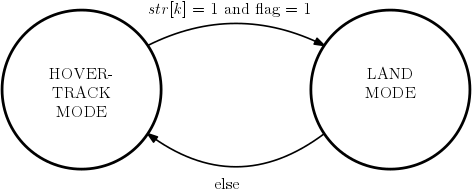
\includegraphics[width=\linewidth]{mixed_model.png}
    \caption{} \label{fig:mixed_model}
  \end{subfigure}%
  \hspace*{\fill}   % maximize separation between the subfigures
  \begin{subfigure}{0.5\textwidth}
    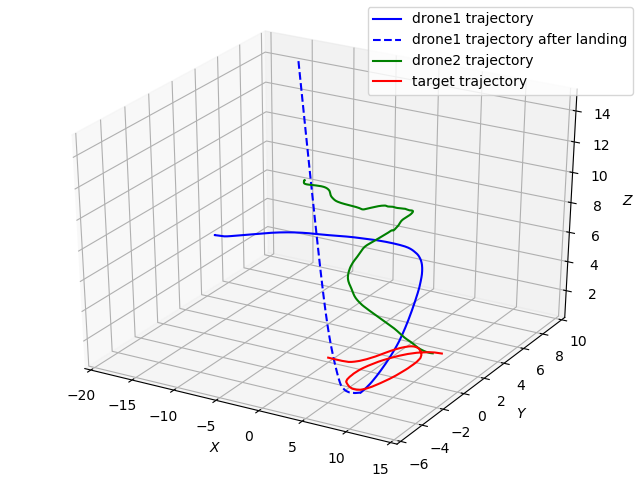
\includegraphics[width=\linewidth]{twist_multi_coord.png}
    \caption{} \label{fig:twist_multi_coord}
  \end{subfigure}%
  \hspace*{\fill}   % maximizeseparation between the subfigures
\caption{(a) A combined model showing both the collaborative strategies mentioned above for UAV index k (b) The final two-level cooperation allowing two UAVs land on a target moving along a curved path} \label{fig:model}
\end{figure}

\section{Results}\label{sec:results}
This section demonstrates the usage of the above proposed strategies for target tracking and autonomous landing. We validate our results in simulation using Gazebo-ROS. In the single UAV tests we start with the UAV 8m behind the rover and from a height of 10m. In the multi UAV tests, we start with the UAVs 8m behind the rover and 4m away on either side, at a height of 10m. After landing, we send the UAV to a random goal, to facilitate landing of the next UAV.
\subsection{Baseline Control Model} \label{sec:baseline_results}
To test the efficacy of the controller in ideal conditions, we first begin with tests on the Baseline model. We consider the problem of landing to be similar to target tracking, and hence apply the model to track a helical path of radius having an equation:
\begin{eqnarray}
x = 10cos(t) & 
y = 10sin(t) & 
z = 0.15t
\end{eqnarray}

\begin{figure}[h]
	\centering
	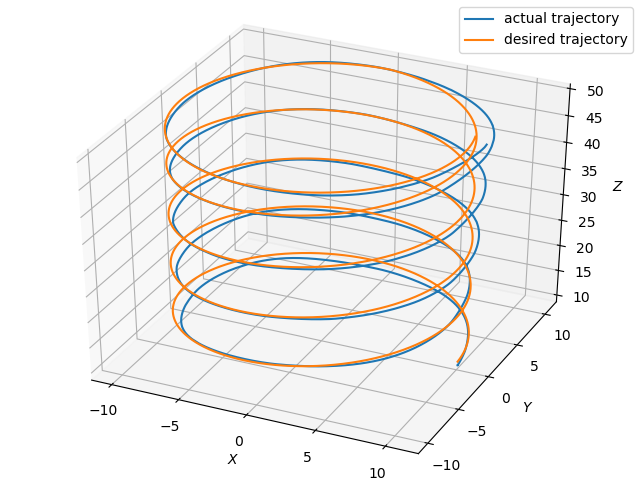
\includegraphics[width=0.49\textwidth]{helix.png}
	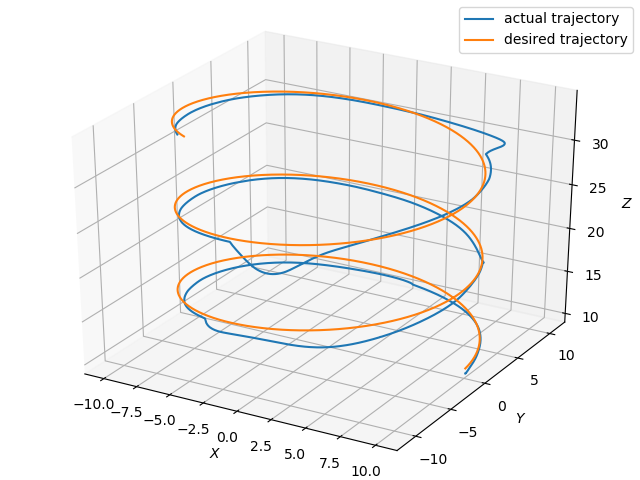
\includegraphics[width=0.49\textwidth]{helix_dist.png}
	\caption{Application of the baseline model to track a helical path (a) without external disturbances (b) with external disturbances}  \label{fig:helix}
\end{figure}

The maximum observed error was $\pm0.4m$ and the minimum was $\pm0.05m$. To test the robustness of the controller, we run tests on a similar path again, but with sudden disturbances. We can observe from Fig.\ref{fig:helix} that the controller is able to regain and track the specified trajectory, even large disturbances.

\begin{figure}
  \begin{subfigure}{0.5\textwidth}
    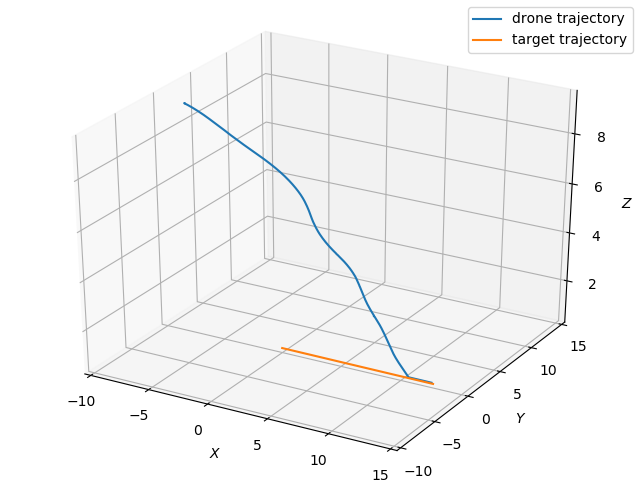
\includegraphics[width=\linewidth]{baseline1.png}
    \caption{} \label{fig:baseline1}
  \end{subfigure}%
  \hspace*{\fill}   % maximize separation between the subfigures
  \begin{subfigure}{0.5\textwidth}
    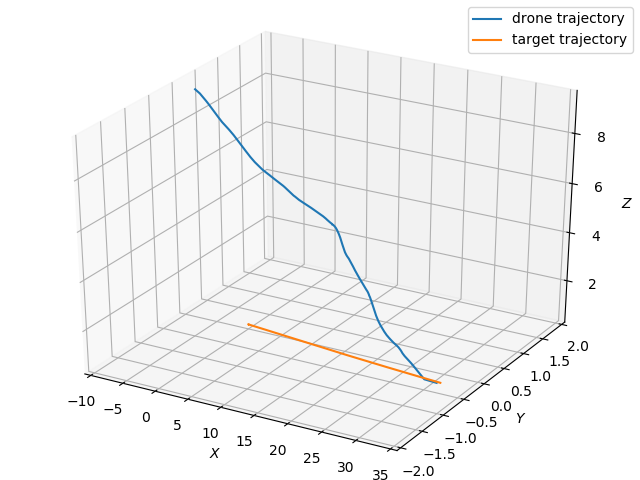
\includegraphics[width=\linewidth]{baseline3.png}
    \caption{} \label{fig:baseline3}
  \end{subfigure}%
  \hspace*{\fill}   % maximizeseparation between the subfigures
  \\
  \begin{subfigure}{0.5\textwidth}
    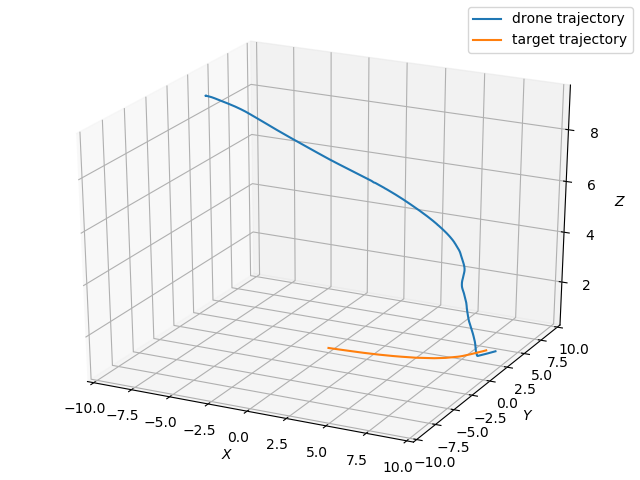
\includegraphics[width=\linewidth]{curve10.png}
    \caption{} \label{fig:curve10}
  \end{subfigure}%
  \hspace*{\fill}   % maximize separation between the subfigures
  \begin{subfigure}{0.5\textwidth}
    \includegraphics[width=\linewidth]{step_curve.png}
    \caption{} \label{fig:step_curve}
  \end{subfigure}%
  \hspace*{\fill}   % maximizeseparation between the subfigures
  \\
  \begin{subfigure}{0.5\textwidth}
    \includegraphics[width=\linewidth]{oscillate.png}
    \caption{} \label{fig:oscillate}
  \end{subfigure}%
  \hspace*{\fill}   % maximize separation between the subfigures
  \begin{subfigure}{0.5\textwidth}
    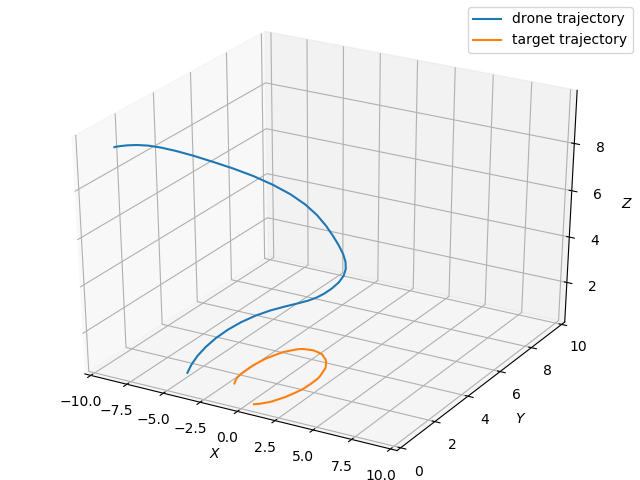
\includegraphics[width=\linewidth]{fail.png}
    \caption{} \label{fig:fail}
  \end{subfigure}%
  \hspace*{\fill}   % maximizeseparation between the subfigures  
\caption{Experimensts using the Baseline controller to land the UAV on a target moving with (a) 1m/s velocity (b) 3m/s velocity (c) circle of radius 10m (d) a staircase-like curve of width 3m (e) sine wave-like curve (f) circle of radius 2m} \label{fig:baseline_land}
\end{figure}

We now apply the Baseline control to the task of autonomous landing, for different scenarios as in Fig.\ref{fig:baseline_land} using: 
\begin{equation}
Q = \begin{bmatrix}
10+\frac{e_{x}^{2}}{|0.5e_{z}^{2}|} & 0 & 0 & 0 & 0 & 0 & 0\\
0 & \frac{150\dot{e}_{x}}{0.01(|e_{x}|+|e_{z}|)} & 0 & 0 & 0 & 0 & 0\\
0 & 0 & 10+\frac{e_{y}^{2}}{|0.5e_{z}^{2}|} & 0 & 0 & 0 & 0\\
0 & 0 & 0 & \frac{150\dot{e}_{y}}{0.01(|e_{x}|+|e_{z}|)} & 0 & 0 & 0\\
0 & 0 & 0 & 0 & 1 + \frac{30e_{z}}{\sqrt{0.1(e_{x}^{2}+e_{y}^{2})}} & 0 & 0\\
0 & 0 & 0 & 0 & 0 & \frac{1}{e_{z}} & 0\\
0 & 0 & 0 & 0 & 0 & 0 & \frac{10}{e_{z}}\\
\end{bmatrix}
\end{equation}
and 
\begin{equation}
R = \begin{bmatrix}
100 & 0 & 0 & 0\\
0 & 100 & 0 & 0\\
0 & 0 & 100 & 0\\
0 & 0 & 0 & 500
\end{bmatrix}
\end{equation}

We can observe from Fig.\ref{fig:baseline1} and Fig.\ref{fig:baseline3} that the UAV is able to land accurately on a target moving on a straight line. We then use the controller for landing when the target moves in a curved trajectory and see its feasiblity from Fig \ref{fig:curve10} and Fig.\ref{fig:step_curve}. We can observe that, although the landing was successful, there exists small closing errors when landing on such curved paths. To further test the controller on more challenging trajectories, we use it to try and land on suddenly changing paths for the target. We observe from Fig.\ref{fig:oscillate} that the UAV lands on the edge of the target plate, while in Fig.\ref{fig:fail}, it misses the target. This is because of the small-radius turns made by the rover, which makes it difficult to land upon. 

\subsection{Vision-only model}

\begin{figure}[h]
\begin{subfigure}{0.33\textwidth}
    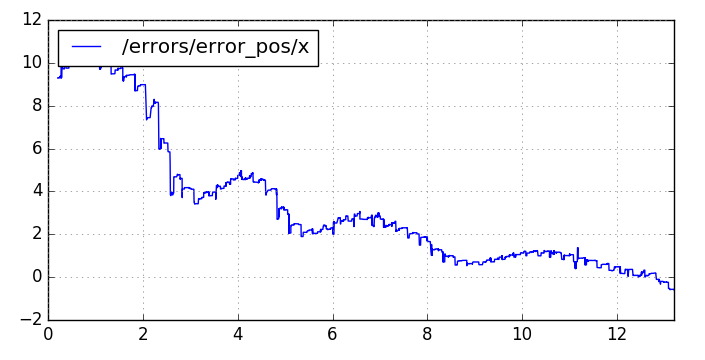
\includegraphics[width=\linewidth]{error_pos_x.png}
    \caption{} \label{fig:errorx}
  \end{subfigure}%
  \hspace*{\fill}   % maximize separation between the subfigures
  \begin{subfigure}{0.33\textwidth}
    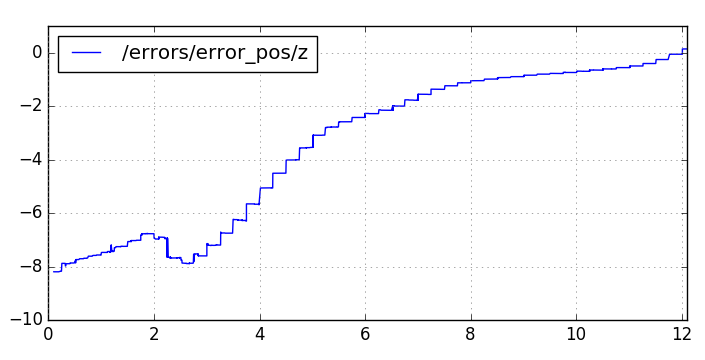
\includegraphics[width=\linewidth]{error_pos_z.png}
    \caption{} \label{fig:errorz}
  \end{subfigure}%
  \hspace*{\fill}   
  \begin{subfigure}{0.33\textwidth}
    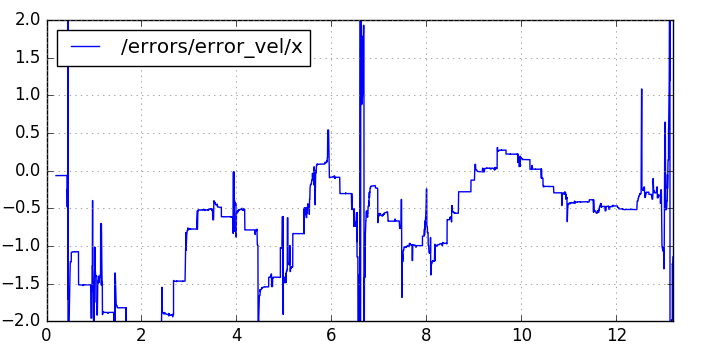
\includegraphics[width=\linewidth]{error_vel_x.png}
    \caption{} \label{fig:error_vel}
  \end{subfigure}%
  \hspace*{\fill} 
 \caption{Errors (a) in position along X direction (b) in position along Z direction (c) in velocity along X direction between the rover and drone while landing. The velocity of the rover is 1m/s.} \label{fig:errors}
\end{figure}

Here we present the results from testing the vision-based controller. The results are show in Fig.\ref{fig:errors} and Fig.\ref{fig:vision_land}. Fig \ref{fig:errors} shows the errors in position along X and Z axes, and the error in velocity along the X axis betweeen the UAV and target, as the rover moves with a velocity of 1m/s along the X axis. We can observe from \ref{fig:errorx} that the error in X decreases rapidly to 0, with some peaks. These peaks arise due to the deceleration of the UAV, so that the velocity of the target can be matched during the time of landing. The error in Z decreases along with decrease in error along X, although not as rapidly, as seen from Fig.\ref{fig:errorz}. This is because as we descend, the FOV from the camera decreases, making it easier to lose the target. Hence, to prevent this from happening, we descend along Z smoothly and slower than along X. For the vision-based tests we use:


\begin{equation}
Q = \begin{bmatrix}
1+\frac{100e_{x}^{2}}{|e_{z}^{2}|} + \frac{50}{||e_{x}|-1|} + \frac{100}{|e_{x}|} & 0 & 0 & 0 & 0 & 0 & 0\\
0 & \frac{20\dot{e_{x}}e_{z}}{0.01|e_{x}|} & 0 & 0 & 0 & 0 & 0\\
0 & 0 & 1+\frac{100e_{y}^{2}}{|e_{z}^{2}|} + \frac{50}{||e_{y}|-1|} + \frac{100}{|e_{y}|} & 0 & 0 & 0 & 0\\
0 & 0 & 0 & \frac{20\dot{e_{y}}e_{z}}{0.01|e_{y}|} & 0 & 0 & 0\\
0 & 0 & 0 & 0 & 1 + \frac{30e_{z}}{\sqrt{0.01(e_{x}^{2}+e_{y}^{2})}} & 0 & 0\\
0 & 0 & 0 & 0 & 0 & \frac{1}{e_{z}} & 0\\
0 & 0 & 0 & 0 & 0 & 0 & \frac{10}{e_{z}}\\
\end{bmatrix}
\end{equation}
and 
\begin{equation}
R = \begin{bmatrix}
75000 & 0 & 0 & 0\\
0 & 75000 & 0 & 0\\
0 & 0 & 800 & 0\\
0 & 0 & 0 & 500
\end{bmatrix}
\end{equation}

\begin{figure}[H]
  \begin{subfigure}{0.5\textwidth}
    \includegraphics[width=\linewidth]{vel1.png}
    \caption{} \label{fig:vel1}
  \end{subfigure}%
  \hspace*{\fill}   % maximize separation between the subfigures
  \begin{subfigure}{0.5\textwidth}
    \includegraphics[width=\linewidth]{vel2.png}
    \caption{} \label{fig:vel2}
  \end{subfigure}%
  \hspace*{\fill}   % maximizeseparation between the subfigures
  \\
  \begin{subfigure}{0.5\textwidth}
    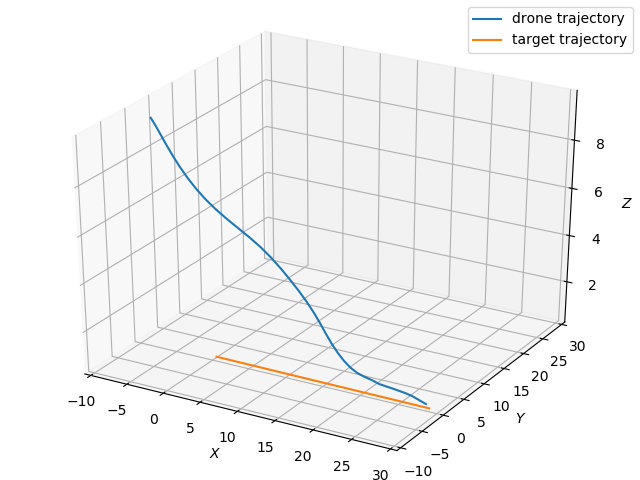
\includegraphics[width=\linewidth]{vel3.png}
    \caption{} \label{fig:vel3}
  \end{subfigure}%
  \hspace*{\fill}   % maximize separation between the subfigures
  \begin{subfigure}{0.5\textwidth}
    \includegraphics[width=\linewidth]{vel4.png}
    \caption{} \label{fig:vel4}
  \end{subfigure}%
  \hspace*{\fill}   % maximizeseparation between the subfigures
  \\
  \begin{subfigure}{0.5\textwidth}
    \includegraphics[width=\linewidth]{step_vision.png}
    \caption{} \label{fig:step_vision}
  \end{subfigure}%
  \hspace*{\fill}   % maximize separation between the subfigures
  \begin{subfigure}{0.5\textwidth}
    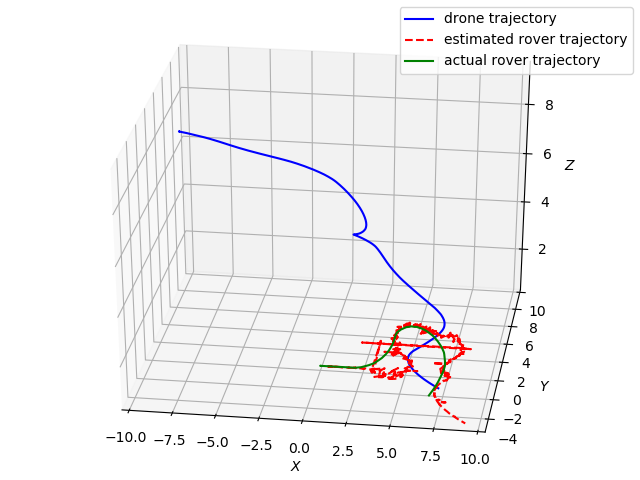
\includegraphics[width=\linewidth]{oscillate_vision.png}
    \caption{} \label{fig:oscillate_vision}
  \end{subfigure}%
  \hspace*{\fill}   % maximizeseparation between the subfigures  
\caption{Vision based landing of the UAV on the target moving along (a) a straight line with velocity 1m/s (b) a straight line with velocity 2m/s (c) a straight line with velocity 3m/s (d) a straight line with velocity 4m/s (e) a staircase like trajectory with step widht 3m and length 5m (f) a sine like curve with amplitude 5m} \label{fig:vision_land}
\end{figure}

\newpage
\subsection{Coordination Strategies}
Here we present the results from the cooperative strategies presented in \ref{sec:coop}. We begin with the coordination algorithm for swerving target, move on to the multiple target landing, and finally combine both to show the UAVs landing on trajectories which were not previously feasible.
\subsubsection{Cooperative Strategy for Swerving Targets}\label{sec:coop1_results}
\begin{figure}[h]
  \begin{subfigure}{0.5\textwidth}
    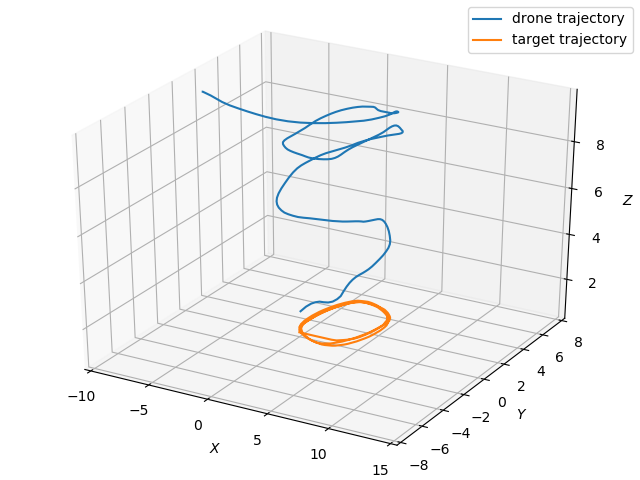
\includegraphics[width=\linewidth]{square_coord.png}
    \caption{} \label{fig:square_coord}
  \end{subfigure}%
  \hspace*{\fill}   % maximize separation between the subfigures
  \begin{subfigure}{0.5\textwidth}
    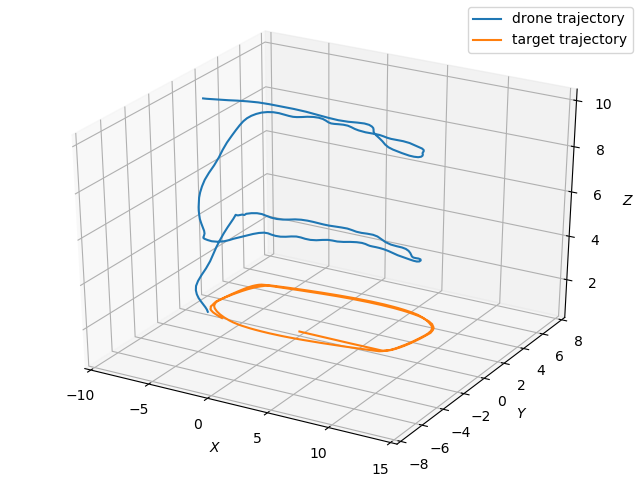
\includegraphics[width=\linewidth]{tight_square_coord.png}
    \caption{} \label{fig:tight_square_coord}
  \end{subfigure}%
  \hspace*{\fill}   % maximizeseparation between the subfigures
  \\
  \begin{subfigure}{0.5\textwidth}
    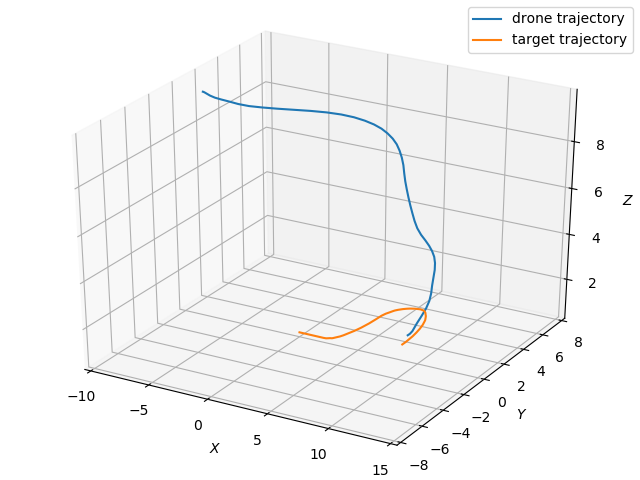
\includegraphics[width=\linewidth]{oscillate_coord.png}
    \caption{} \label{fig:oscillate_coord}
  \end{subfigure}%
  \hspace*{\fill}   % maximize separation between the subfigures
  \begin{subfigure}{0.5\textwidth}
    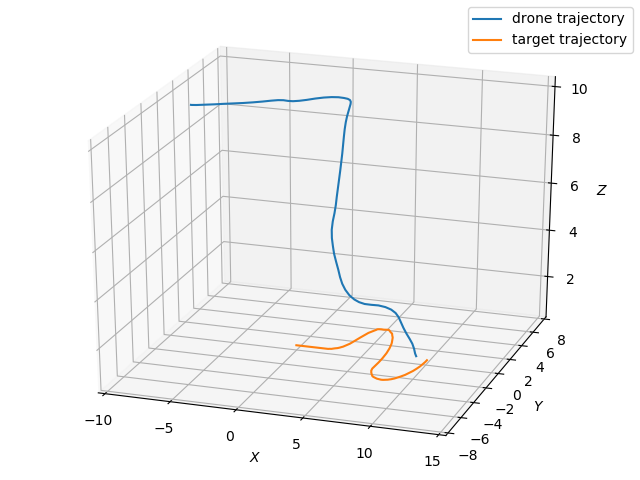
\includegraphics[width=\linewidth]{oscillate_coord_3.png}
    \caption{} \label{fig:oscillate_coord_3}
  \end{subfigure}%
  \hspace*{\fill}   % maximizeseparation between the subfigures
  \\
\caption{Trajectories of UAV and target as the target moves along (a) a square of length 5m (b) a rectangle of length 8m and width 5m (c) a sine like curve with amplitude 5m (d) a sine like curve with amplitude 3m} \label{fig:Coordination_curve}
\end{figure}

Fig.\ref{fig:Coordination_curve} shows the results of the coordination strategy used to land the UAV using the baseline controller, on the target as it moves along different curved trajectories. To test the controller on challenging conditions, we make the UAV land when the target moves along the shorter path of its trajectory. In Fig.\ref{fig:square_coord}, Fig.\ref{fig:oscillate_coord}, and Fig.\ref{fig:oscillate_coord_3}, the UAV is made to land when the rover moves perpendicular to the X axis, and track otherwise. In Fig.\ref{fig:tight_square_coord} the UAV is asked to land as the rover moves along the side of length 3m, and track as the target moves along the 8m side. We observe that by making the UAV only track the target while holding its altitude instead of attempting to land makes it possible for the UAV to adapt to the changes in the rover's path more easily. This allows the UAV to land on paths with length as short as 2m which was previously infeasible.

\newpage
\subsubsection{Multiple UAV Landing}\label{sec:coop2_results}
\begin{figure}[H]
  \begin{subfigure}{0.5\textwidth}
    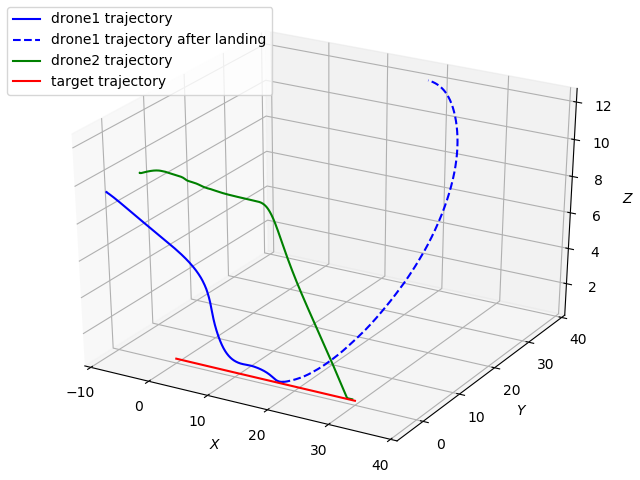
\includegraphics[width=\linewidth]{straight_multi.png}
    \caption{} \label{fig:straight_multi}
  \end{subfigure}%
  \hspace*{\fill}   % maximize separation between the subfigures
  \begin{subfigure}{0.5\textwidth}
    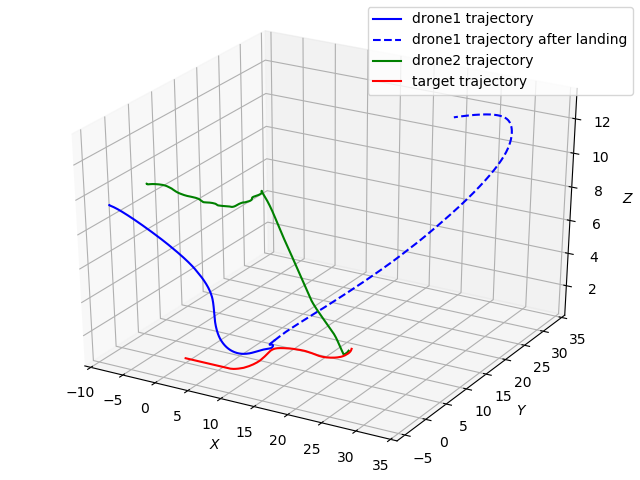
\includegraphics[width=\linewidth]{step_multi.png}
    \caption{} \label{fig:step_multi}
  \end{subfigure}%
  \hspace*{\fill}   % maximizeseparation between the subfigures
\caption{Multiple agents landing on a target (a) moving in a straight line (b) moving along a step like trajectory with length 8m in either direction} \label{fig:multiple}
\end{figure}

Here we show the cooperative strategy for landing multiple UAVs on the target, as discussed in Sec.\ref{sec:coop2}. Although there is no restriction on the controller we could use, to test both controllers for this setting and increase simulation speeds, we use vision-only based landing for drone1 and baseline control for drone2. The results of the experiments are shown in Fig.\ref{fig:multiple}. We can observe that the vision-based model is smoother than the baseline model, and it can be observed more clearly in Fig.\ref{fig:multiple_coord}. This can be attributed to the fact that the $R$ matix in the vision model has substantially larger entries than the ones in the baseline model. As a result we penalize accelerations and decelerations more in the vision based system, and thus the trajectory generated is smoother. Consequently, the vision-based model is able to track and land on slower and more smoother target trajctories than the baseline model. In this work we have presented the results for only two UAVs and a single rover. However the presented algorithms can be extended to multiple such UAVs and targets, with some minor modifications as suggested in Sec.\ref{sec:conclusions}

\subsubsection{Two-Level Cooperation}
\begin{figure}[H]
  \begin{subfigure}{0.5\textwidth}
    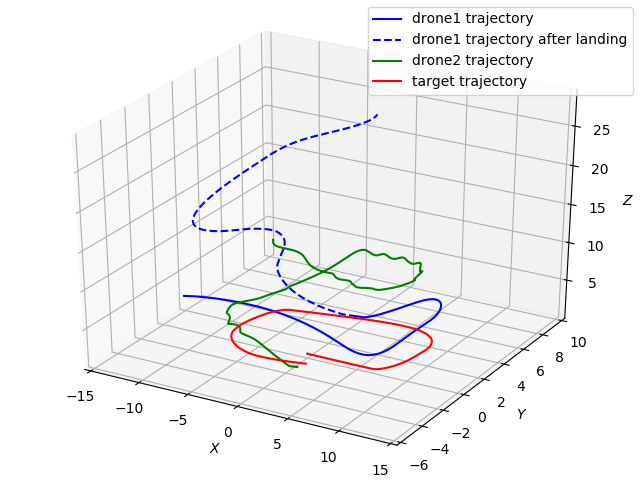
\includegraphics[width=\linewidth]{tight_square_multi_coord.png}
    \caption{} \label{fig:tight_square_multi_coord}
  \end{subfigure}%
  \hspace*{\fill}   % maximize separation between the subfigures
  \begin{subfigure}{0.5\textwidth}
    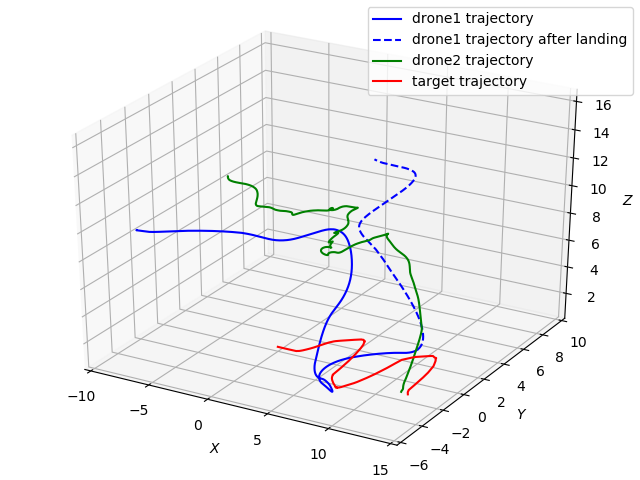
\includegraphics[width=\linewidth]{oscillate_multi_coord.png}
    \caption{} \label{fig:oscillate_multi_coord}
  \end{subfigure}%
  \hspace*{\fill}   % maximizeseparation between the subfigures
\caption{Multiple agents scheduling} \label{fig:multiple_coord}
\end{figure}

Here we present the final desired results from the two-level cooperation scheme presented. We use the model presented in Fig.\ref{fig:mixed_model}, and as in Sec.\ref{sec:coop2_results} we use a vision based model for drone1 and the baseline model for drone2. The results of the simulations are presented in Fig.\ref{fig:multiple_coord}.


\section{Conclusions}\label{sec:conclusions}
This paper presents a SDRE-based controller for precise autonomous landing. The controller is then extended to a vision-only based landing scheme. Cooperative strategies to land on swiftly moving targets, and for multi-UAV landings are discussed. Extensive simulation results of the proposed framework is presented. Future work involves using collision avoidance algorithms for the multi-UAV landing setting, and extending the problem as a scheduling question. The effects of continuous and/or time-varying winds on the controller is also to be tested. Further incorporating the UAV dynamics into the controlled would make it more robust for a particular drone. We also wish to extend the proposed system for fixed-wing landings.

\bibliography{refs}

\end{document}
